\pagebreak
\section{Front End}
\subsection{Business Delegate}

The team working on the frontend needs to have ready to use functions, without having to know how the backend works or how to connect to it. This is why we create a Business Delegate, a class made by the backend team which gives the functions useful for the frontend application.

In our case, the backend team need to give two things. The first is a subset of the package used in the server containing the Facade interface and the Entities classes. This is needed because the backend methods will return these classes, which are just objects with some fields, getters/setters and equals/hashCode functions (cleaned of the extra injections used in the backend). They are implementing Serializable, which makes easy for them to be shared remotely (DTO). To make JNDI work, we need to put these files, which are in common with the server, in the same package structure as the server itself, otherwise the connection will return the ClassNotFoundException. 
\footnote{https://stackoverflow.com/questions/13701041/remote-ejb-call-class-not-found-\\exception/13703265}

The second thing the backend team will give to the frontend one is a folder containing the business delegate class and a service locator. The frontend team will need only to interface with the business delegate class to do their job. The service locator for the client is not used to find the different EJBs inside the project, but to interface with the server: in this case, we need the \textit{InitialContext} to have some properties to tell him where to connect (properties given by the function \textit{getJndiProperties()}). We can see how also here the Service Locator is a Singleton.

\begin{figure}[H]
  \centering
  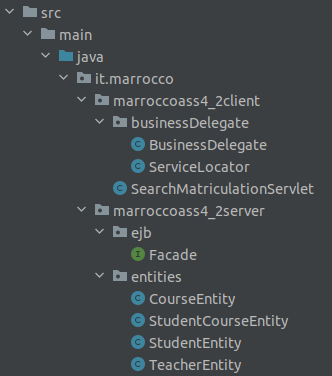
\includegraphics[width=0.3\columnwidth]{client_folder_structure.png}
  \caption{The structure of the Client project}
\end{figure}

\pagebreak
\begin{lstlisting}[language=java, caption={BusinessDelegate}]
  public class BusinessDelegate {
      Facade facadeEJB;
      public BusinessDelegate() {
          try {
              String jndiName = "ejb:/MarroccoAss4_2-Server-1.0-SNAPSHOT/FacadeEJB!it.marrocco.marroccoass4_2server.ejb.Facade";
              facadeEJB = (Facade) ServiceLocator.getService(jndiName);
          } catch (NamingException e) {
              System.out.println("Naming exception: " + e.getMessage());
              e.printStackTrace();
              throw new RuntimeException(e);
          }
      }

      public StudentEntity getSingleStudent(int matriculation) {
          return facadeEJB.getSingleStudent(matriculation);
      }

      public List<StudentCourseEntity> getStudentCourses(int matriculation) {
          return facadeEJB.getStudentCourses(matriculation);
      }

      public List<TeacherEntity> getStudentTeachers(int matriculation) {
          return facadeEJB.getStudentTeachers(matriculation);
      }
  }
\end{lstlisting}

\pagebreak
\begin{lstlisting}[language=java, caption={Client ServiceLocator}]
  public class ServiceLocator {
      private static HashMap<String, Object> cache;

      static {
          cache = new HashMap<String, Object>();
      }

      private static Properties getJndiProperties() {
          Properties jndiProperties=new Properties();
          jndiProperties.put(Context.INITIAL_CONTEXT_FACTORY, "org.wildfly.naming.client.WildFlyInitialContextFactory");
          jndiProperties.put(Context.PROVIDER_URL,"http-remoting://localhost:8080");
          jndiProperties.put(Context.URL_PKG_PREFIXES, "org.jboss.ejb.client.naming");
          jndiProperties.put("jboss.naming.client.ejb.context", true);

          return jndiProperties;
      }

      public static Object getService(String jndiName) throws NamingException {
          Object service = cache.get(jndiName);
          if (service == null) {
              InitialContext context = new InitialContext(getJndiProperties());
              service = context.lookup(jndiName);
              cache.put(jndiName, service);
          }
          return service;
      }
  }
\end{lstlisting}

\pagebreak
\subsection{Html Pages}
First we create the index.jsp file, which is a simple form that has a field for the matriculation number and two checks, one for each page, to choose what to get from the server.

The form will redirect to our servlet, which will take the matriculation number from the request body. It will then instantiate the class BusinessDelegate made by the backend team in the \textit{init()} method, call its functions to get the data necessary from the server and use it to create HTML parts.

\begin{lstlisting}[language=java, caption={SearchMatriculationServlet}]
  @WebServlet(name = "searchMatriculation", value = "/searchMatriculation")
  public class SearchMatriculationServlet extends HttpServlet {
      BusinessDelegate bd;
  
      @Override
      public void init() {
          try {
              bd = new BusinessDelegate();
              System.out.println("Connection working");
          } catch(RuntimeException e) {
              System.out.println("Cannot get connection to server");
          }
      }
  
      public String formatStudentEntity(StudentEntity s) {
          return "<h1>" + s.getSurname() + " " + s.getName() + " (" + s.getMatriculation() + ")</h1>";
      }
  
      public String getStudentPageElement(int matriculation) {
          StudentEntity s = bd.getSingleStudent(matriculation);
          if (s == null) return "<h1>Student was not found</h1>";
          String html = formatStudentEntity(s);
          html += "<h2>Courses:</h2>";
          try {
              html += "<ul>";
              List<StudentCourseEntity> sc = bd.getStudentCourses(matriculation);
              if (sc == null) return "<h1>Error getting the Student Courses</h1>";
              for (StudentCourseEntity c : sc) {
                  html += "<li>" + c.getCourse().getName();
                  if(c.getGrade() != null)
                      html +=  " (grade = " + c.getGrade() + ")";
                  html += "</li>";
              }
              html += "</ul>";
          } catch (Exception e ) {
              System.out.println("error: " + e.getMessage());
              html += "<h3>error<h3>";
          }
          return html;
      }
  
      public String getAdvisoryPageElement(int matriculation) {
          StudentEntity s = bd.getSingleStudent(matriculation);
          if (s == null) return "<h1>Student was not found</h1>";
          String html = formatStudentEntity(s);
          html += "<h2>Advisors:</h2>";
          try {
              html += "<ul>";
              List<TeacherEntity> sc = bd.getStudentTeachers(matriculation);
              if (sc == null) return "<h1>Error getting the Student Teachers</h1>";
              for (TeacherEntity t : sc) {
                  html += "<li>" + t.getSurname() + " " + t.getName() + "</li>";
              }
              html += "</ul>";
          } catch (Exception e ) {
              System.out.println("error: " + e.getMessage());
              html += "<h3>error<h3>";
          }
          return html;
      }
  
      public void doPost(HttpServletRequest request, HttpServletResponse response) throws IOException {
          int matriculation;
          try {
              matriculation = Integer.parseInt(request.getParameter("matriculation"));
          } catch (NumberFormatException e) {
              response.sendRedirect("");
              return;
          }
          boolean showStudentPage = request.getParameter("studentPage") != null;
          boolean showAdvisoryPage = request.getParameter("advisoryPage") != null;
  
          String html = "";
          try {
              if (showStudentPage) html += getStudentPageElement(matriculation);
              if (showAdvisoryPage) html += getAdvisoryPageElement(matriculation);
          } catch (Exception e) {
              System.out.println("Error in fetching data");
              html += "<h1>Error in fetching data</h1>";
              html += "<p>"+e.getMessage()+"</p>";
          }
  
          response.setContentType("text/html");
          PrintWriter out = response.getWriter();
          out.println("<html><head><title>Matriculation "+matriculation+"</title></head><body>");
          out.println(html);
          out.println("<a href='index.jsp'>Go back</a>");
          out.println("</body></html>");
          out.close();
      }
  }
\end{lstlisting}

\pagebreak
\subsection{Pages Images}

\begin{figure}[H]
  \centering
  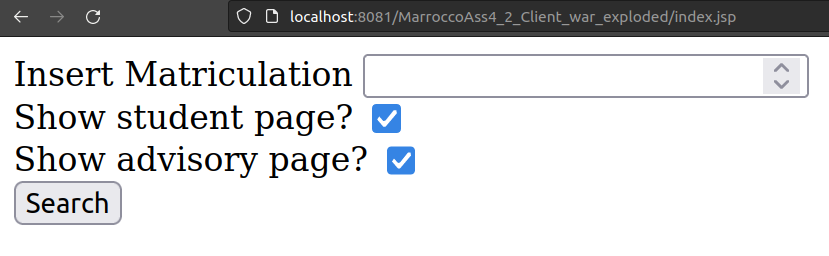
\includegraphics[width=0.7\columnwidth]{index2.png}
  \caption{The starting page}
\end{figure}

\begin{figure}[H]
  \centering
  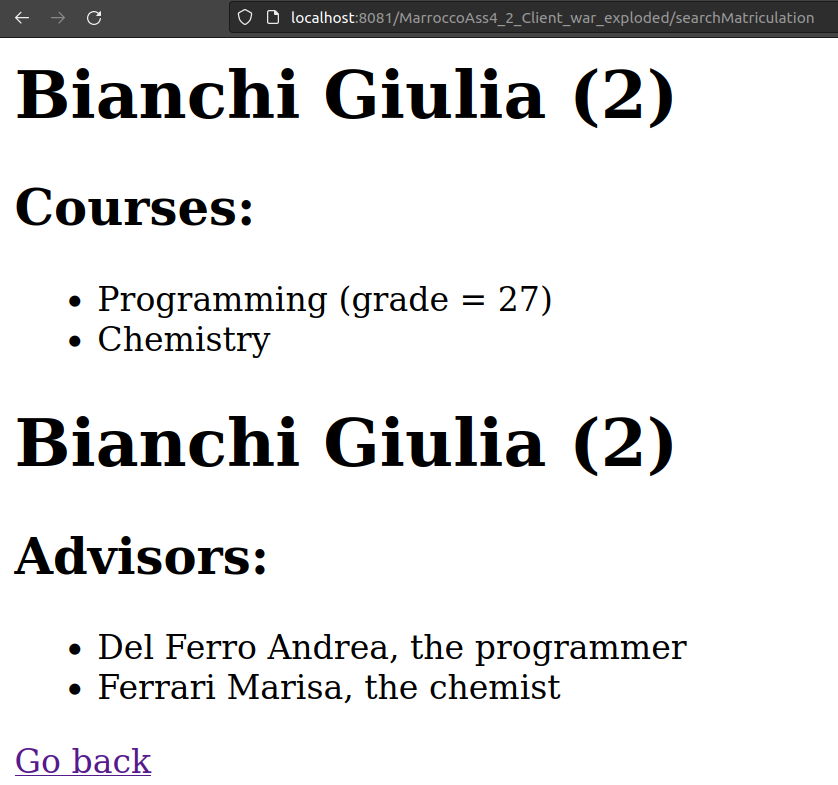
\includegraphics[width=0.7\columnwidth]{full_page2.png}
  \caption{The servlet page when both checks are set, showing both requested pages}
\end{figure}

\begin{figure}[H]
  \centering
  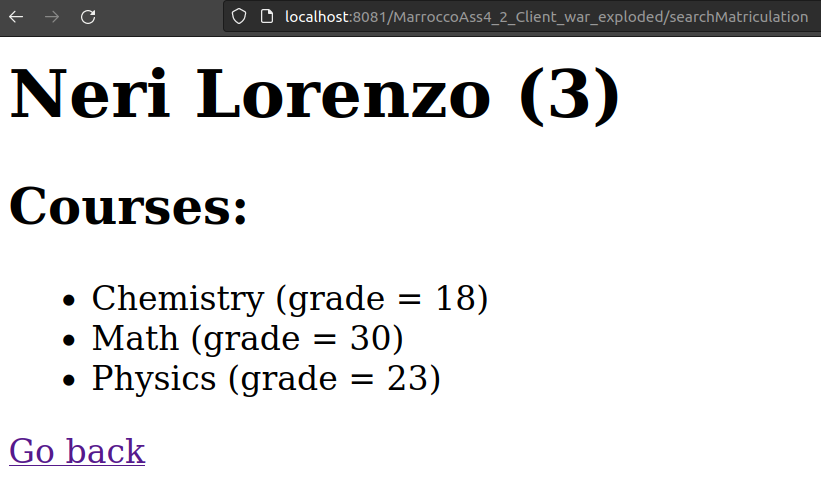
\includegraphics[width=0.7\columnwidth]{only_one_page2.png}
  \caption{The servlet page with only the courses page}
\end{figure}

\begin{figure}[H]
  \centering
  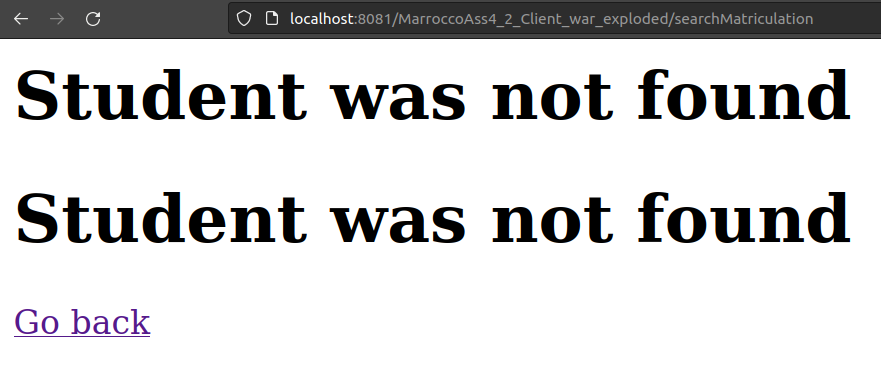
\includegraphics[width=0.7\columnwidth]{no_student_found2.png}
  \caption{The servlet page when a non existant student is searched}
\end{figure}